\section{Multilingual Usable Security and Remediation (RQ4)}
\label{sec:usable}

Automated verification fails to improve security if software engineers and auditors cannot interpret its findings or translate them into corrective code~\cite{sasse_usable_sec, acar_developers, wash_developers}. In non-Anglophone emerging economies, technical English security jargon creates severe cognitive friction. To evaluate whether evidence-grounded, localized diagnostic reporting enhances human comprehension and remediation efficiency (RQ4), we conducted a controlled human-subjects experiment ($N=60$).

\subsection{Experimental Design, Counterbalancing, and Ethics}
\label{sec:usable:design}

We conducted a within-subjects study approved by the Institutional Review Board at Mymensingh Engineering College (Protocol \#MEC-CSE-IRB-2025-0812) with written informed consent from all 60 participants. We recruited 60 professional participants from Dhaka's technology and banking sectors, stratified into: (1) 30 Android software engineers ($4.8 \pm 2.1$ years professional experience); and (2) 30 IT compliance auditors and risk officers ($5.2 \pm 2.6$ years experience). All were native Bengali speakers with professional working proficiency in English.

Following a balanced $3 \times 3$ Latin Square crossover design~\cite{box_latin_square}, participants were randomized into three treatment groups ($n=20$ each), counterbalancing three reporting conditions across three equivalent defect scenarios (transport security, cryptographic storage, and PII leakage)~\cite{wohlin_experimentation}:
\textit{Condition A (Raw Diagnostic)}: Conventional vulnerability scanner outputs (e.g., MobSF raw traces with CWE tags and generic English warnings).
\textit{Condition B (Evidence-Grounded English)}: Structured English report detailing the 7-tuple mapping, 5-state verdict, bytecode witness provenance, and remediation code.
\textit{Condition C (Evidence-Grounded Localized Bengali)}: Localized Bengali report presenting official statutory gazette text, evidence witnesses, and remediation guidance in native technical Bengali.

\begin{figure*}[t]
\centering
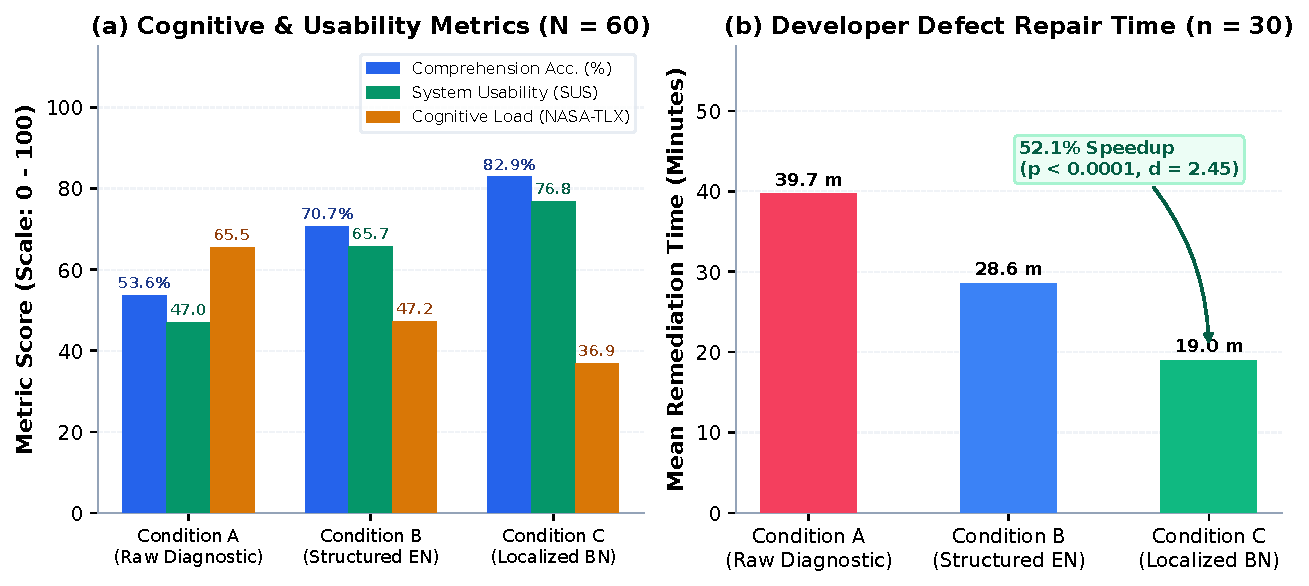
\includegraphics[width=0.66\textwidth]{figures/fig5_usable_security_results.pdf}
\caption{\textbf{Controlled Human-Subjects Usable Security Evaluation Results ($N=60$)}: (a) Usability metrics across Condition A (Raw Scanner Trace), Condition B (Evidence-Grounded English), and Condition C (Evidence-Grounded Localized Bengali). Bengali reporting increases comprehension accuracy from $53.6\%$ to $82.9\%$ ($p < 0.0001, d = 2.15$), elevates SUS scores to $76.8$ ($d = 2.38$), and reduces NASA-TLX cognitive load from $65.5$ to $36.9$ ($d = 2.02$). (b) Developer defect repair time ($n_1 = 30$), showing a $52.1\%$ reduction in remediation time (from $39.7$ to $19.0$ minutes, $p < 0.0001, d = 2.45$).}
\label{fig:usable_security_results}
\end{figure*}

\subsection{Dependent Evaluation Metrics}
\label{sec:usable:metrics}

Tasks were evaluated against four standardized dependent variables: (1) \textit{Comprehension accuracy} measured via a 10-item objective technical comprehension questionnaire; (2) \textit{System Usability Scale (SUS, 0--100)}~\cite{brooke_sus}; (3) \textit{NASA-TLX Cognitive Workload (0--100)}~\cite{hart_tlx}; and (4) \textit{Time-to-remediate}, defined as the total wall-clock duration in minutes from task initiation to patch submission (capped at a 45-minute cutoff, evaluated on an intent-to-treat basis including failed attempts for the developer cohort $n_1 = 30$). To ensure cross-task equivalence across the $3 \times 3$ Latin Square rotation, all three remediation scenarios were calibrated to identical 3-to-5 line modification complexity requiring replacement of insecure cipher transformations, network security configurations, or intent flags.

\begin{table*}[t]
\caption{Controlled Human-Subjects Usable Security Evaluation Results ($N=60$): Decomposing Structured Reporting (A vs. B) from Linguistic Localization (B vs. C)}
\label{tab:usability_results}
\centering
\small
\resizebox{\textwidth}{!}{%
\begin{tabular}{lcccccc}
\toprule
\textbf{Evaluation Metric} & \textbf{Cond. A (Raw)} & \textbf{Cond. B (EN)} & \textbf{Cond. C (BN)} & \textbf{A vs. B (Struct.)} & \textbf{B vs. C (Local.)} & \textbf{A vs. C (Total)} \\
\midrule
\textbf{Comprehension Accuracy (\%)} & $53.6\% \pm 15.9$ & $70.7\% \pm 13.4$ & $\mathbf{82.9\% \pm 10.9}$ & $p < 0.001$ ($d = 1.16$) & $p < 0.001$ ($d = 1.00$) & $p < 0.001$ ($d = 2.15$) \\
\textbf{System Usability Scale (SUS)} & $47.0 \pm 14.8$ & $65.7 \pm 11.6$ & $\mathbf{76.8 \pm 9.8}$ & $p < 0.001$ ($d = 1.41$) & $p < 0.001$ ($d = 1.04$) & $p < 0.001$ ($d = 2.38$) \\
\textbf{NASA-TLX Cognitive Load} & $65.5 \pm 15.8$ & $47.2 \pm 12.6$ & $\mathbf{36.9 \pm 12.3}$ & $p < 0.001$ ($d = 1.28$) & $p < 0.001$ ($d = 0.83$) & $p < 0.001$ ($d = 2.02$) \\
\midrule
\multicolumn{7}{l}{\textit{Developer Cohort Only ($n_1 = 30$):}} \\
\textbf{Time-to-Remediate (min)} & $39.7 \pm 10.4$ & $28.6 \pm 8.7$ & $\mathbf{19.0 \pm 5.9}$ & $p < 0.001$ ($d = 1.16$) & $p < 0.001$ ($d = 1.29$) & $p < 0.001$ ($d = 2.45$) \\
\textbf{Patch Success Rate (\%)} & $46.7\%$ ($14/30$) & $70.0\%$ ($21/30$) & $\mathbf{86.7\%}$ ($26/30$) & McNemar $p = 0.016$ & McNemar $p = 0.063$ & McNemar $p < 0.001$ \\
\bottomrule
\end{tabular}%
}
\vspace{1mm}
\footnotesize \raggedright \textit{Statistical Notes:} Paired two-tailed $t$-tests with Bonferroni correction ($\alpha_{\text{adj}} = 0.0167$) and paired Cohen's $d$ for continuous variables. McNemar's exact binomial test for paired binary patch success ($n_1 = 30$).
\end{table*}

\subsection{Quantitative Results and Statistical Decomposition}
\label{sec:usable:results}

Repeated-measures omnibus ANOVA confirmed significant main effects of diagnostic condition across all dependent variables ($F(2, 118) > 94.2, p < 0.0001$ for comprehension, SUS, and TLX across $N=60$; $F(2, 58) = 78.4, p < 0.0001$ for time-to-remediate across the developer cohort $n_1=30$). Pairwise post-hoc comparisons were evaluated via paired two-tailed $t$-tests with Bonferroni correction ($\alpha_{\text{adj}} = 0.0167$) (Table~\ref{tab:usability_results} and Figure~\ref{fig:usable_security_results}):

\paragraph{Structured Evidence Effect (Condition A vs. B)} Transitioning from unstructured scanner dumps to structured English reports improved comprehension by $+17.1$ percentage points (pp) ($53.6\% \rightarrow 70.7\%, t(59) = 7.57, p < 0.0001, d = 1.16$) and reduced developer repair time by $27.9\%$ ($39.7 \rightarrow 28.6$ minutes, $t(29) = 6.48, p < 0.0001, d = 1.16$). Paired analysis confirmed a statistically significant improvement in developer patch success from $46.7\%$ ($14/30$) to $70.0\%$ ($21/30$) (McNemar's exact binomial test, discordant pairs $b=7, c=0, p = 0.0156$). The complete absence of regressions ($c=0$) reflects the scaffolding: Condition B provided verified code diffs, enabling 7 previously failing developers to successfully patch defects. We explicitly note that providing remediation code diffs in Conditions B and C measures the developer's ability to \textit{comprehend and correctly apply a recommended fix}, rather than independently conceiving code repairs from diagnostic traces alone.

\paragraph{Linguistic Localization Effect (Condition B vs. C)} Presenting diagnostics in native technical Bengali with authentic legal text yielded an additional $+12.2$ pp in comprehension ($70.7\% \rightarrow 82.9\%, t(59) = 7.29, p < 0.0001, d = 1.00$), accelerated defect repair by an additional $9.6$ minutes ($28.6 \rightarrow 19.0$ minutes, $33.6\%$ speedup over English, $t(29) = 6.89, p < 0.0001, d = 1.29$), and reduced subjective cognitive load by $10.3$ points ($47.2 \rightarrow 36.9, d = 0.83$). Developer patch success rose to $86.7\%$ ($26/30$), exhibiting a positive trend over English (discordant pairs $b=5, c=0, p = 0.0625$), while the cumulative gain over raw scanner output (Condition A vs. C) was highly significant ($46.7\% \rightarrow 86.7\%$, discordant pairs $b=12, c=0, p = 0.0005$). The monotonic nested progression ($14 \subset 21 \subset 26; c=0$) demonstrates that removing technical language barriers resolves lingering ambiguity without introducing regressions. However, because our design contrasted structured English against structured Bengali (omitting an unstructured Bengali baseline), this comparison estimates the joint effect of linguistic localization and statutory gazette framing rather than pure language translation in isolation.

\noindent\textbf{Translation Fidelity and Practical Significance.}\label{sec:usable:translation} To ensure translation fidelity, statutory clauses were drawn from authoritative texts: CSA clauses from the official Government Gazette (Act XXVII of 2023), BB-CSF clauses from central bank BRPD circulars, and PDPA clauses from the cabinet-approved draft bill. Technical descriptions were vetted via forward-and-backward translation with our panel's Supreme Court advocate. In practice, cutting remediation time from $28.6$ to $19.0$ minutes and elevating patch correctness from $70.0\%$ to $86.7\%$ substantially reduces defect leakage into production while bridging communication barriers between legal counsel and engineering teams ($d \approx 2.02 - 2.45$ across A-to-C)~\cite{cohen_kappa, wohlin_experimentation}.
